\chapter{Reconstruction as an Auxiliary Task for Generative Modeling}
\label{chap:chapter2}

\begin{chapterabstract}
	In this chapter, we propose an approach for conditioning a GAN model to reconstuct images from a very sparse set of randomly-positioned pixels known beforehand. This approach, based on a Maximum A Posteriori estimation, takes the form of an explicit auxiliary reconstruction task which adds to the GAN objective as an additional loss term. Complemented with the PacGAN variant for training GANs, this approach enables the generation of diverse samples from a sparse pixel map. As opposed to the more classical Conditional GAN approach, this auxiliary task is interpretable and a hyperparameter allows to control the importance of the conditioning in the learning process. We evaluate our approach on the classical MNIST, FashionMNIST and CIFAR10 datasets, as well as a custom-made texture dataset. Finally,  we apply this approach to a task of geostatistical simulation.
\end{chapterabstract}

 \section{Image Reconstruction with Generative Models}

Image reconstruction is the task of completing an image from a very small subset of the pixels. Such source data can usually be found in domains where the measurement process is very noisy or where measurements are expensive. This task differs from image inpainting since the source data is usually unstructured and very scarce, as in this chapter we will consider randomly scattered measurements of less than a percent of the image. While our discussion focus on image reconstruction, it is noteworthy to mention that this applies to other kinds of signals.

The task of image reconstruction is challenging since very few information is available for use. To overcome this lack of information, generative models such as GANs leverage on existing datasets to learn the distribution of the real images. By conditioning the learned distribution, a GAN could learn to generate an image while enforcing the constraint that the pixels known beforehand must remain similar in the generated image.

Similarly as in the GAN setup, we denote  by $X \in \setX$ a random variable and $x$ its realization. Let $p_X$ be the distribution of $X$ over $\setX$ and $p_X(x)$ be its evaluation at $x$. Similarly $p_{X|Y}$ represents the distribution of $X$ conditioned on the random variable $Y \in \setY$. 

We denote by $x \in \setX = [-1, 1]^{n\times p\times c}$  (see Figure \ref{fig:digit}) an image sampled from an unknown distribution $p_X$  and a sparse matrix  $y \in  \setY = [-1, 1]^{n\times p\times c}$ (Figure \ref{fig:pixelwise_gen}) as the given constrained pixels. The problem  then consists in finding a generative model $G$ with inputs $z$ (a random vector sampled from a known distribution $p_Z$ over the space $\setZ$) and constrained pixel values $y \in  [-1, 1]^{n\times p\times c}$ that maps the distribution $p_Z$ onto the distribution of the real samples $p_X$ while enforcing the constraints $y$ (see Figure \ref{fig:image_completion}), which is to learn the conditional distribution $p_{X|Y,Z}.

\begin{figure}[t]
	\centering
	\begin{subfigure}[t]{0.33\textwidth}
		\centering
		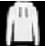
\includegraphics[width=3cm]{chapter2/fashion_sample.jpg}
		\caption{Original \\ Image}
		\label{fig:digit}
	\end{subfigure}\begin{subfigure}[t]{0.33\textwidth}
		\centering
		
\includegraphics[width=3cm]{chapter2/fashion_sample_inpainting.jpg}
		\caption{Inpainting\\Input}
		\label{fig:inpainting}
	\end{subfigure}\begin{subfigure}[t]{0.33\textwidth}
		\centering
		
\includegraphics[width=3cm]{chapter2/fashion_sample_pixel.jpg}
		\caption{Constraint\\Map}
		\label{fig:pixelwise_gen}
	\end{subfigure}
	\caption{Difference between regular inpainting (\ref{fig:inpainting}) and the problem undertaken in this work (\ref{fig:pixelwise_gen}) on a real sample (\ref{fig:digit}).}
	\label{fig:image_completion_task}
\end{figure}

	
Introduction to the problem of image reconstruction, definitions and formulation

Related works : CGAN, AmbientGAN, UNIR,  Compressed Sensing with Meta-Learning

Limitations of these models

\section{Conditional generation as a Maximum A Posteriori estimation}
Approche de l'article NeuCom :

Formulation as a Maximum A Posteriori Estimation, assumptions (normal error)

Construction of the loss term using bayes rule and least squares 

PacGAN for keeping the diversity

\section{Experimental evaluation and application to underground soil generation}

Datasets : MNIST/FashionMNIST/CelebA/Texture

Evaluation : MSE/FID; Epoch  selection criterion

Architectures : Appendix ? DCGAN + SGAN (encoder-decoder)

Results : visible trade-off, good fidelity overall

Application to hydro-geology : subsurface dataset

Evaluation : MSE/HOG+LBP

\section{Conclusion}

Objective reached : tuneable loss, pixel-wise, keeping diversity

Applications in hydro-geology : papier Eric

Future works : other distributions (modelling error using Laplacian, beta or Poisson distributions)
